\documentclass[12pt,hyperref,a4paper,UTF8]{ctexart}
\usepackage{HDUReport}
\usepackage{listings}
\usepackage{xcolor}
\usepackage{graphicx}
\usepackage{setspace}
\usepackage{float}
\setstretch{1.5} % 设置全局行距为1.5倍

\usepackage{enumitem} % 载入enumitem包以便自定义列表环境
\setlist[itemize]{itemsep=0pt, parsep=0pt} % 设置itemize环境的项目间距和段落间距

\setmainfont{Times New Roman} % 英文正文为Times New Roman


\usepackage{tikz}
\usetikzlibrary{shapes.geometric, arrows}
\usetikzlibrary{positioning, arrows.meta}
\usetikzlibrary{calc}
%封面页设置
{   
    %标题
    \title{ 
        \vspace{1cm}
        \heiti \Huge \textbf{《电磁波与电磁场实验》作业报告} \par
        \vspace{1cm} 
        \heiti \Large {\underline{实验3：分布参数滤波器的设计、仿真、优化和分析}   }     
    }

    \author{
        \kaishu\Large 指导教师\ \dlmu[9cm]{吴爱婷}  \\
        \kaishu\Large 学生姓名\ \dlmu[9cm]{陈文轩} \\ %学院
        \kaishu\Large 学生学号\ \dlmu[9cm]{23040447} \\ %
        \kaishu\Large 学生班级\ \dlmu[9cm]{23186011} \\ %班级
        \kaishu\Large 学生专业\ \dlmu[9cm]{智能硬件与系统(电子信息工程)} \qquad  \\ %学号
        \kaishu\Large 实验日期\ \dlmu[9cm]{2025.10.20} \qquad \\
         %姓名 
    }
        
    \date{\today} % 默认为今天的日期，可以注释掉不显示日期
}
%%------------------------document环境开始------------------------%%
\begin{document}

%%-----------------------封面--------------------%%
\cover
\thispagestyle{empty} % 首页不显示页码
%%------------------摘要-------------%%
%\newpage
%\begin{abstract}




%\end{abstract}

%\thispagestyle{empty} % 首页不显示页码

%%--------------------------目录页------------------------%%
% \newpage
% \tableofcontents
% \thispagestyle{empty} % 目录不显示页码

%%------------------------正文页从这里开始-------------------%
\newpage
\setcounter{page}{1} % 让页码从正文开始编号

%%可选择这里也放一个标题
%\begin{center}
%    \title{ \Huge \textbf{{标题}}}
%\end{center}

\section{实验目的}

1.通过此次实验，我们需要熟悉微带线电路的仿真过程和注意事项，理解微带线的特性和各种参数指标。

2.本次实验我们需要用到 TX Line 工具，需要熟练掌握 MWO 提供 TX Line 的使用方法和技巧。

3.设计分布参数低通滤波器。


\section{实验内容}


1. 采用微带传输线设计低通滤波器；

2. 设计指标：

截止频率：\(500MHz\)；

通带内：\(S_{21} \sim 0.5 dB\)，\(S_{11} \sim 20 dB\)；

阻带内：\(900MHz\) 以上 \(S_{21} \sim 30 dB\)；

3. 仿真频段 \(100MHz \cdot 1000MHz\)，步长 10MHz，要求电路对称，端口阻抗 \(50\) 欧姆，电路阶数不限，以最少阶数为佳。


\subsection{主要实验步骤}

1.创建工程，设置工程属性

2.画原理图，选择优化变量；画原理图时，利用TXline工具，求得高阻抗（100$\Omega$）、50$\Omega$、低阻抗（$\Omega$）的各个对应的微带线宽度$W$（5.2mm、1.9mm、0.4mm），将此代入到微带线电路的MLIN的参数设置中。

\begin{figure}[H]
  \centering
  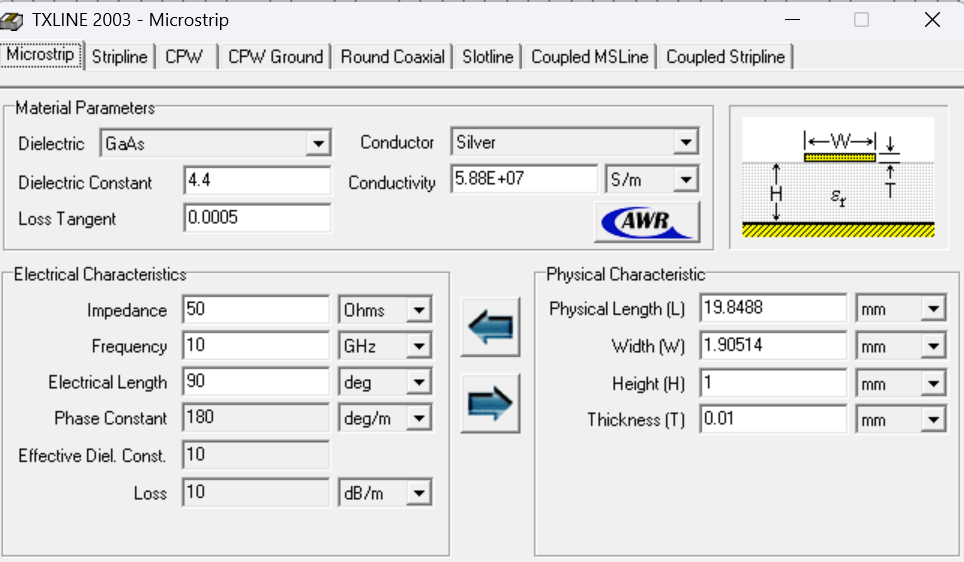
\includegraphics[width=1\textwidth]{figures/TXline.png}
  \caption{利用TXline求解微带线宽度界面}
  \label{fig:example}
\end{figure}


\begin{figure}[H]
  \centering
  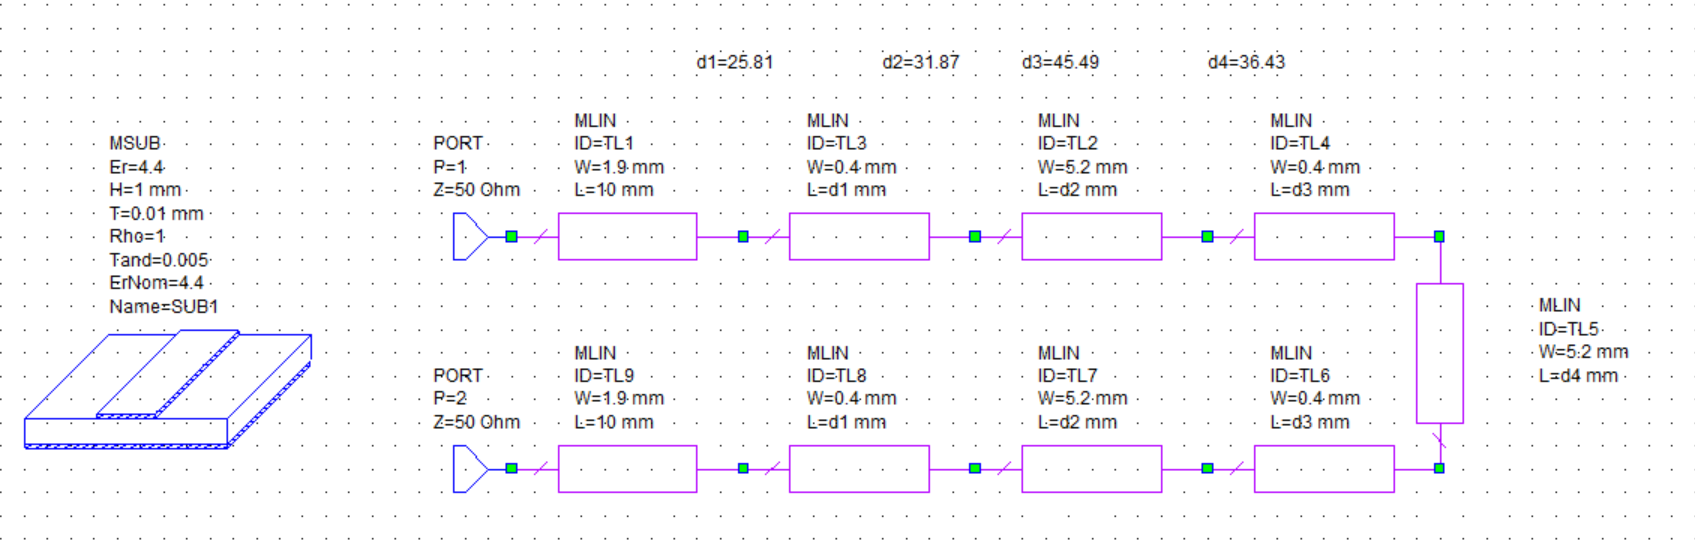
\includegraphics[width=1\textwidth]{figures/电路.png}
  \caption{微带线电路原理图}
  \label{fig:example}
\end{figure}

3.添加输出界面图及测量参量

4.选择优化目标，进行优化目标设定

\begin{figure}[H]
  \centering
  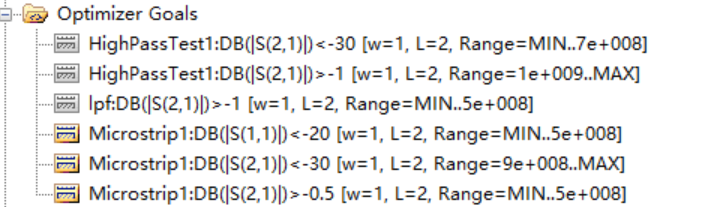
\includegraphics[width=1\textwidth]{figures/约束设计.png}
  \caption{优化目标设计}
  \label{fig:example}
\end{figure}


5.运行结果，对结果进行优化

\begin{figure}[H]
  \centering
  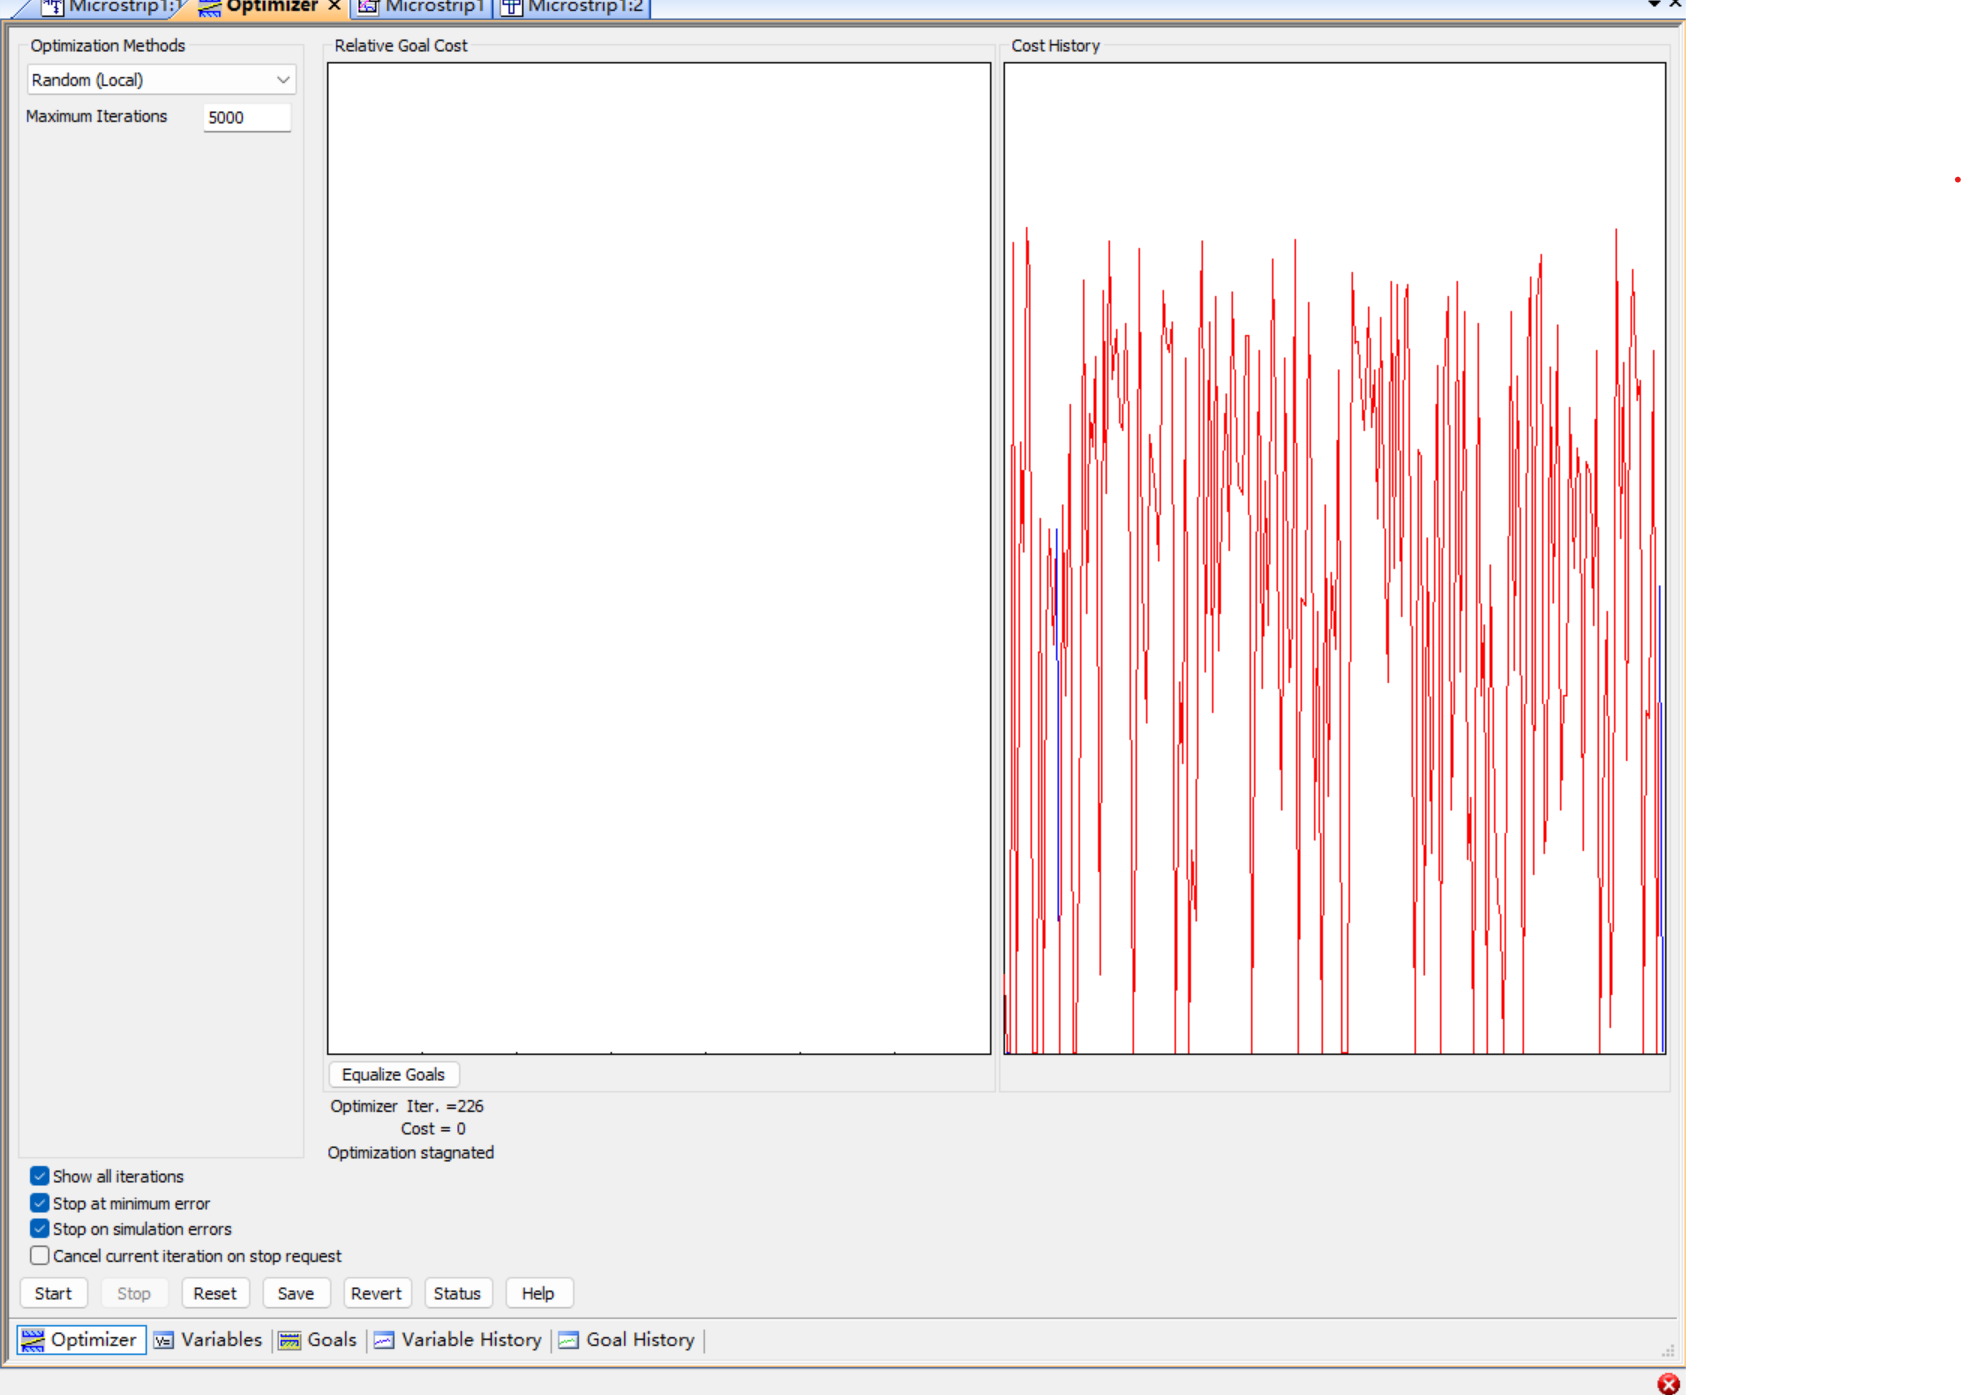
\includegraphics[width=1\textwidth]{figures/COST.png}
  \caption{优化后，最后的cost=0}
  \label{fig:example}
\end{figure}


6.生成版图

\begin{figure}[H]
  \centering
  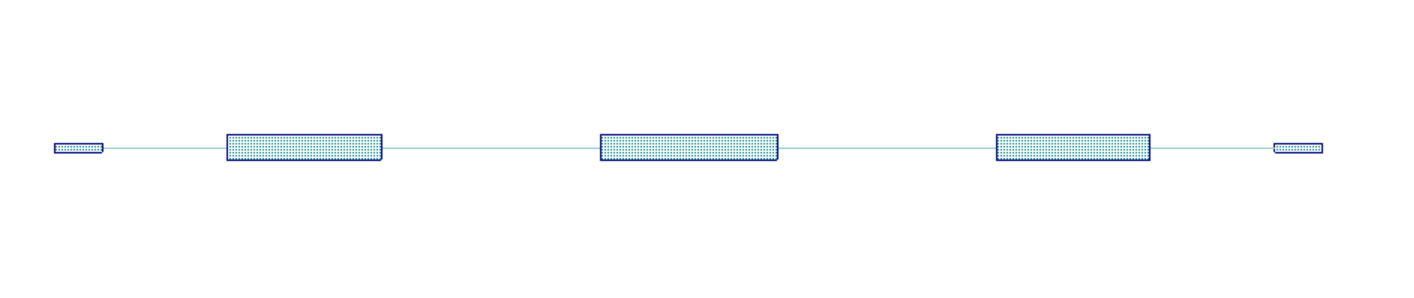
\includegraphics[width=1\textwidth]{figures/版图.png}
  \caption{微带线设计的版图}
  \label{fig:example}
\end{figure}



\section{总结}

本次实验成功完成了基于微带传输线的分布参数低通滤波器设计、仿真与优化。通过使用MWO软件和TX Line工具，初步理解了微带线特性及其在滤波器设计中的应用。

\subsection{目标完成}

通过MWO的优化功能，最终实现了优化目标cost = 0，表明所有设计指标均得到满足。优化过程主要调整了各段微带线的长度参数，使得：

\begin{itemize}
    \item 通带内（$f < 500$MHz）：插入损耗$S_{21} > -0.5$dB，反射系数$S_{11} < -20$dB，信号传输良好；
    \item 阻带内（$f > 900$MHz）：插入损耗$S_{21} < -30$dB，有效抑制高频信号；
    \item 电路采用对称结构设计，保证了良好的端口匹配和频率响应特性。
\end{itemize}

\subsection{实验收获}

1. 初步认识了TX Line工具的使用方法，能够根据特性阻抗要求快速计算微带线几何尺寸；

2. 初步理解了分布参数滤波器的设计原理，认识到微带线长度和阻抗对滤波特性的影响；

3. 初步熟悉了MWO软件的优化流程，学会了设置优化目标和约束条件，实现了自动化设计优化；

4. 通过版图生成，了解了实际的微带线样式；


\end{document}